\documentclass[18pt]{article}
\usepackage{listings}
\usepackage{fontspec}
\usepackage[bookmarks=true, pdfborder={0 0 0}]{hyperref}
\usepackage{blindtext}
\usepackage{caption}
\usepackage{amsmath}
\captionsetup[table]{labelformat=empty, labelsep=none}
\usepackage[
inner=3cm,      % Mehr Platz für die Bindung
outer=3cm,      % Standardplatz nach außen
top=3cm,
bottom=3cm
]{geometry}

\usepackage{graphicx}
\graphicspath{{assets/}}

\usepackage{color}
\definecolor{deepblue}{rgb}{0,0,0.5}
\definecolor{deepred}{rgb}{0.6,0,0}
\definecolor{deepgreen}{rgb}{0,0.5,0}


\hypersetup{
	colorlinks=true,      % Rahmen entfernen und Text einfärben
	linkcolor=blue,       % Farbe für interne Verweise (Tabellen, Kapitel, etc.)
	urlcolor=blue,        % Farbe für Web-Adressen
	citecolor=green!60!black % Farbe für Zitate (Dunkelgrün)
}

\DeclareFixedFont{\ttb}{T1}{txtt}{bx}{n}{12} % for bold
\DeclareFixedFont{\ttm}{T1}{txtt}{m}{n}{12}  % for normal

\newfontfamily{\jetbrainsmono}{JetBrains Mono}

% Python style for highlighting
\newcommand\pythonstyle{\lstset{
		language=Python,
		basicstyle=\jetbrainsmono\fontsize{9}{9}\selectfont,
		morekeywords={self},              % Add keywords here
		keywordstyle=\ttb\color{deepblue}\fontsize{9}{9}\selectfont,
		emph={get_device_temp_and_humid, get_luminance, get_motion, display_text, SoftI2C, SSD1306\_I2C, Pin, json, , ADC, DHT22, sleep, collect, mqtt_connect, hexlify, connect, restart_and_reconnect, MQTTClient, reset, check_msg, publish, OSError, osdebug, send_message, can_send_message},
		emphstyle=\ttb\color{deepred}\fontsize{9}{9}\selectfont,  
		stringstyle=\color{deepgreen}\fontsize{9}{9}\selectfont,
		frame=tblr,    
		showstringspaces=false,
		literate={*}{{\raisebox{0.8ex}{$\ast$}}}{1}
}}

% Python environment
\lstnewenvironment{python}[1][]
{
	\pythonstyle
	\lstset{#1}
}
{}

% Python for inline
\newcommand\pythoninline[1]{{\pythonstyle\lstinline!#1!}}

\newcommand\pythonexternal[2][]{{
		\pythonstyle
		\lstinputlisting[#1]{#2}}}

\begin{document}

\begin{titlepage}
	\centering
	\vspace{2cm}
	{\Huge \bfseries Wetterstation ESP32\\}
	\vspace{1cm}
	{\Large \itshape Dokumentation der Entwicklung einer Wetterstation mit dem ESP32\\}
	\vspace{3cm}
	{\bfseries Eingereicht am: 16. Dezember 2025\\}
	\vspace{0.5cm}
	\rule{10cm}{1pt}\\
	\vspace{0.5cm}
	{\bfseries Dieses Dokument wurde mit \LaTeX{} erstellt.\\}
	
	\vfill
	
	\begin{flushleft}
		\large
		\textbf{Autor:} Anthony Timmel\\
		\textbf{Klasse:} Fi24\\
		\textbf{Lernfeld:} 7\\
		\textbf{Lernbereich:} Cyberphysische Systeme\\
	\end{flushleft}
	\vspace{3cm}
	{\large Berufsschule Weißwasser - Informationstechnik}
	
\end{titlepage}
\newpage
\tableofcontents
\newpage

\section{Definition der Schnittstellen}
\subsection[GPIO]{Der Port GPIO}
\subsection[UART]{Der Port UART}
\subsection[I2C]{Der Port I2C}
\subsection[SPI]{Der Port SPI}


\newpage

\section{Aufbau des ESP32}

\begin{figure}[htbp]
	\centering
	% You can drop the extension and path if using \svgpath
	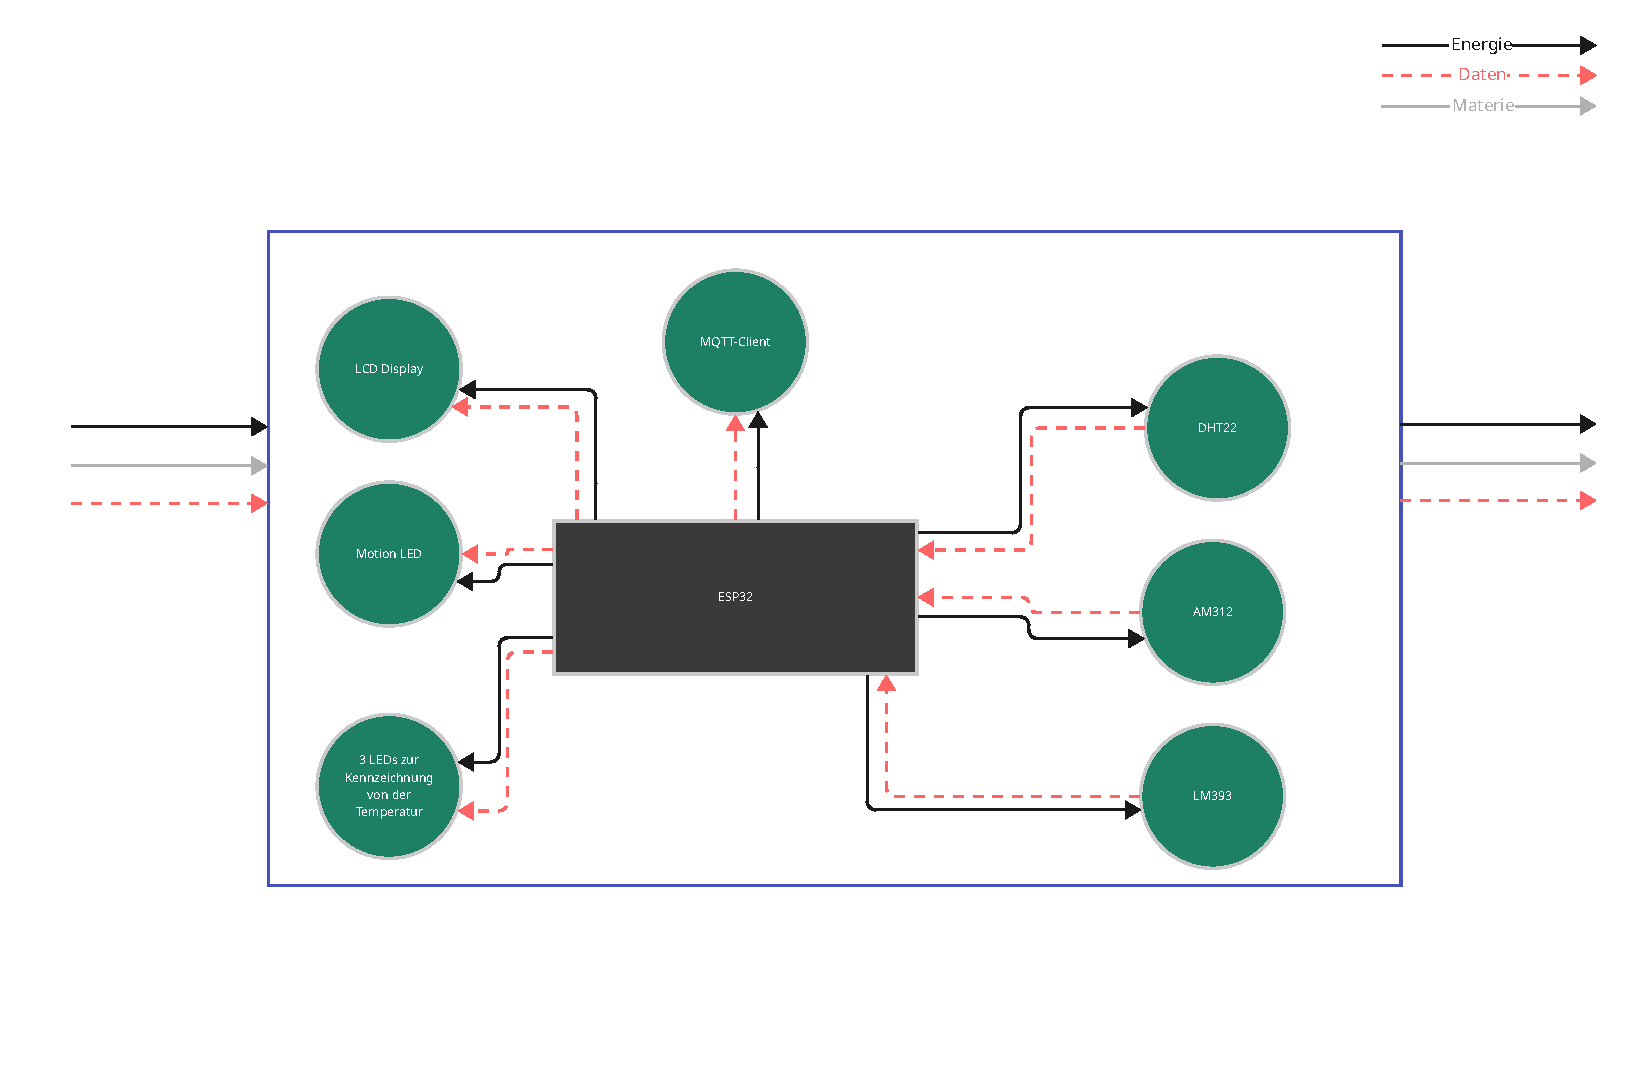
\includegraphics[width=\textwidth]{ESP32_Structure.pdf}
	\caption[width=\textwidth]{ESP32 Internal Structure}
\end{figure}

\begin{figure}
	\centering
	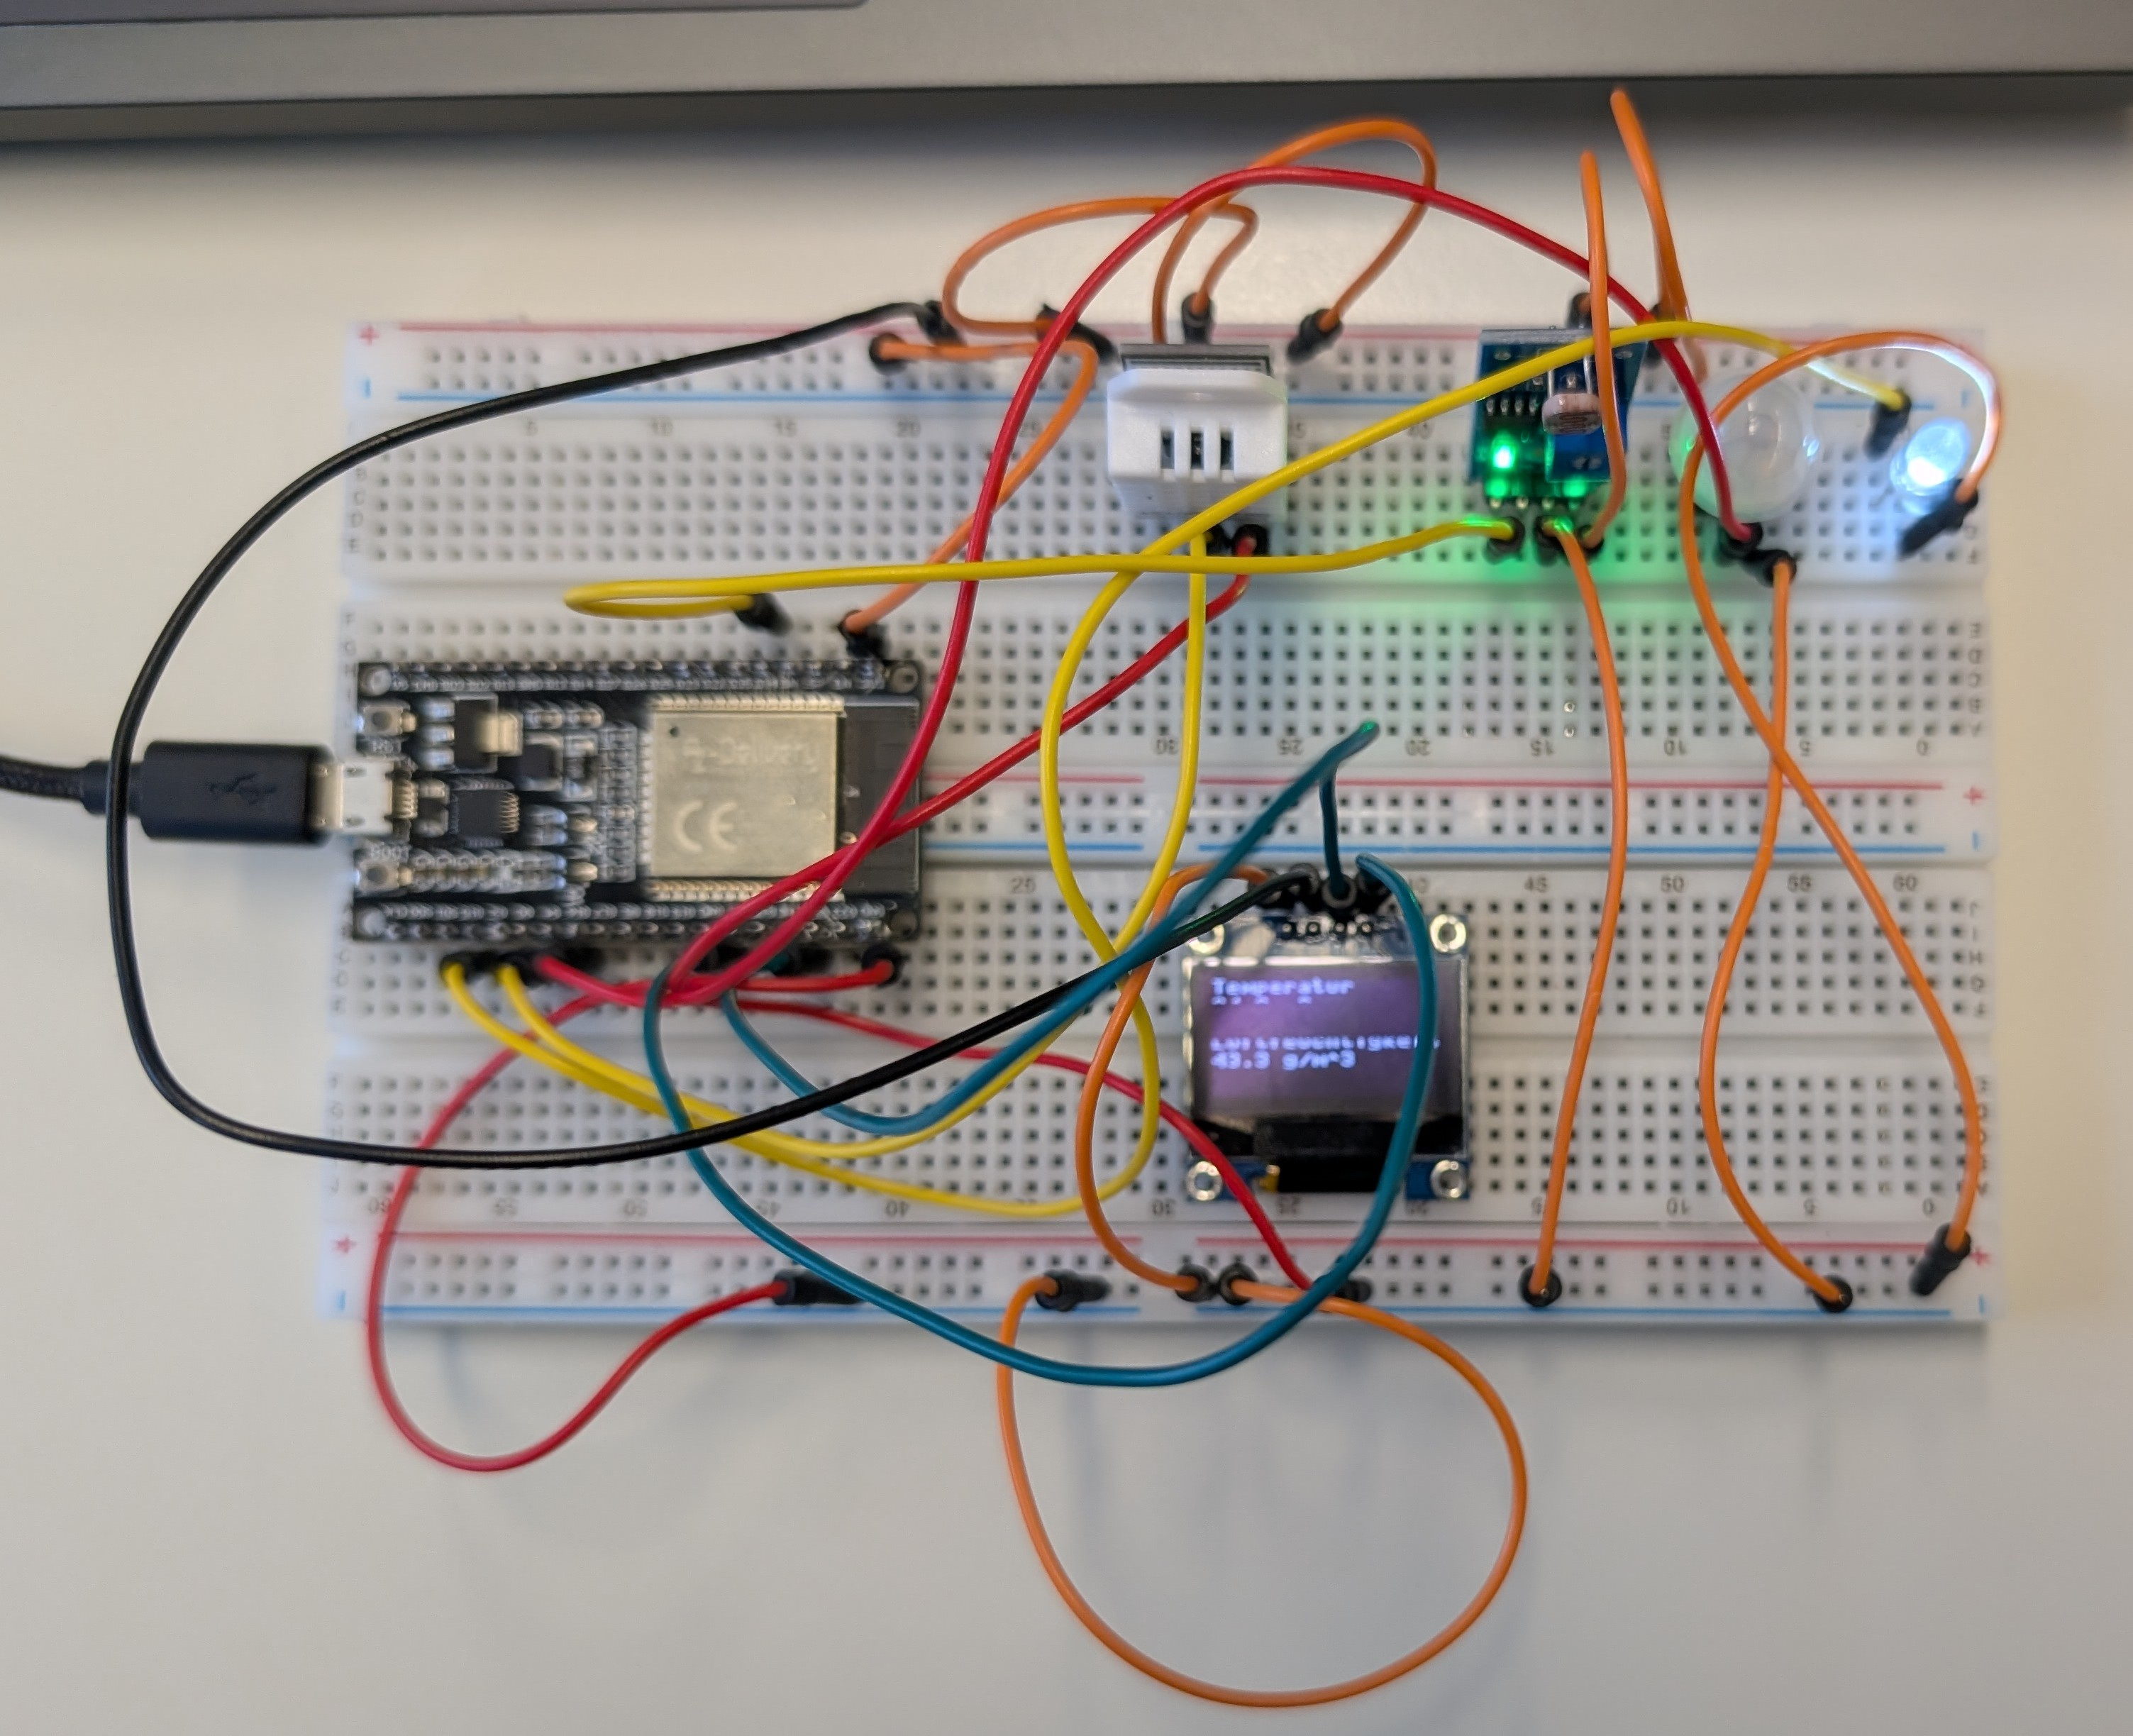
\includegraphics{esp32_top-view.jpg}
	\caption{ESP32 Topansicht}
\end{figure}

\newpage
\section{Aufgabe Teil 1}	
\subsection[Anforderungen]{Anforderungen}
\textbf{Bevor} das cyber-physische System (CPS) in das \textbf{interne} Netzwerk integriert
werden kann sollen sie testen, ob die Möglichkeit besteht mit einem ESP32
als Grundlage des CPS, die Temperatur und die Luftfeuchtigkeit mit einem
Sensor (\textbf{DHT22}) einzulesen und zu verarbeiten. Für die sekündliche
Übermittlung der Daten an den später auszuwertenden MQTT-Client sollen
die Sensorwerte in das Datenformat JSON abgelegt werden.

\textbf{\textit{Zusatz:}} Greifen Sie auf den Inhalt des in MicroPython erstellten JSON-Strings
zu und \textbf{geben} Sie die Sensordaten mit der \pythoninline{print()}-Funktion im Terminal aus.

\vfill

\subsection[Hardware]{Die Vernetzung der Hardware auf dem Steckbrett}

\subsubsection{Bauelemente}

\textbf{ESP32}
\newline
Der \textit{ESP32} befindet sich bereits \textbf{vorinstalliert} auf dem Steckbrett und kann, durch das \textbf{Hinzufügen} des Stromversorgungs- \& Datenübertragungskabels lässt sich die Einheit, von dem Computer aus Steuern.
\renewcommand{\arraystretch}{1.5}
\begin{table}[h!] % [h!] = hier platziere die Tabelle möglichst hier
\centering % Zentriert die Tabelle auf der Seite
\caption{Verteilung der Pin-Nutzung auf dem ESP32} % Beschriftung der Tabelle
\label{tab:teil_1_steckbrett_esp32} % Label für Referenzen
\begin{tabular}{|l|l|} % Definiert 3 Spalten: zentriert, linksbündig, rechtsbündig, mit vertikalen Linien
\hline
Pin & Aufgabe \\
\hline
3V3 & Stromversorgung des Bauteils \\
GND & Die Masse des ESP32 \\
GPIO4 & Universeller Eingangspin für die Messdaten es DHT22 \\
\hline % Horizontale Linie
\end{tabular}
\end{table}
\renewcommand{\arraystretch}{1}
\newline
\newline
\textbf{DHT22}
\newline
Das Erweiterungsmodul \textit{DHT22} ist ein Modul, was es \textbf{ermöglicht}, die Raumtemperatur sowie die Luftfeuchtigkeit in der Umgebung \textbf{festzustellen}.
\renewcommand{\arraystretch}{1.5}
\begin{table}[h!] % [h!] = hier platziere die Tabelle möglichst hier
\centering % Zentriert die Tabelle auf der Seite
\caption{Verteilung der Pin-Nutzung auf dem DHT22} % Beschriftung der Tabelle
\label{tab:teil_1_steckbrett_dht22} % Label für Referenzen
\begin{tabular}{|l|l|} % Definiert 3 Spalten: zentriert, linksbündig, rechtsbündig, mit vertikalen Linien
\hline
Pin & Aufgabe \\
\hline
VCC & Stromversorgung des Bauteils \\
GROUND & Die Masse des DHT22 \\
DATA & Datenübertragungsport für die Messdaten es Bauteils \\
\hline % Horizontale Linie
\end{tabular}
\end{table}
\renewcommand{\arraystretch}{1}

\subsubsection{Vernetzung der Bauelemente}
Der \textit{ESP32} ist mit dem Pin \textbf{ADC2\_0 GPIO4} mit dem \textit{DHT22} \textbf{DATA} Pin verbunden.
Die Stromversorgung des \textit{DHT22} geht über den \textbf{VCC} Pin des Bauteils, dieser ist mit der Stromversorgung von dem \textbf{3V3} Pin des \textit{ESP32} verbunden.
Der \textbf{GROUND} Pin des Bauteils, ist mit der Masse \textbf{GND} des \textit{ESP32} zusammengeschlossen, damit die Schaltung elektrotechnisch Funktionstüchtig werden kann.


\subsection[Programmcode]{Programmcode für den ESP32}

\begin{python}
def get_device_temp_and_humid():
	dht_device = DHT22(Pin(4, Pin.IN))
	dht_device.measure()
	temp = dht_device.temperature()
	humid = dht_device.humidity()

	return temp, humid
\end{python}
\vfill
Mithilfe dieser Funktion, ist es uns möglich, die \textbf{Temperatur} und \textbf{Luftfeuchtigkeit} an dem \textbf{aktuellen Ort} zu bestimmen. Dafür sendet das Modul \textit{DHT22} seine Daten an den Pin \textbf{G4}, diesen aben wir zuvor (\hyperref[tab:teil_1_steckbrett_esp32]{Pinverteilung ESP32}) definiert.

Durch \textbf{DHT22} aus der Datei \textbf{dht} erhalten wir die Möglichkeit, Daten über eine Erweiterung des Protokolls abzugreifen. Dafür haben wir den Input-Pin der DHT22 Klasse \pythoninline{DHT22(Pin(4, Pin.IN))} bei der Initialisierung \textbf{übergeben}. Im Anschluss ist es uns nun möglich, eine Messung \textbf{mithilfe} von \pythoninline{dht_device.measure()} können wir das Modul \textbf{auffordern}, eine Messung der Temperatur sowie Luftfeuchtigkeit vorzunehmen. Im Anschluss \textbf{erhalten} wir die Temperatur sowie Luftfeuchtigkeit über die jeweilige Methode des Objektes und geben diese am Ende der Funktion als \texttt{Pair} zurück.
\newline

\vfill

\begin{python}
while True:
	temp, humid = get_device_temp_and_humid()

	raw_json_object = {
		"Temperatur": temp,
		"Luftfeuchtigkeit": humid
	}

	json_object = json.dumps(raw_json_object)

	print(json_object)
	sleep(1)
\end{python}
\vfill
Mithilfe \textbf{dieser} Schleife, ermöglicht es uns, bestimmte Bauteile \textbf{jede} Sekunde, auf dem \textit{ESP32} abzufragen und im Anschluss, die Daten weiter zu verarbeiten.
Dafür holen wir uns die \textbf{Temperatur} \& \textbf{Luftfeuchtigkeit} über die Funktion \pythoninline{get_device_temp_and_humid()}.
Im Anschluss erstellen wir ein \texttt{Dictionary}, um die Daten später im Programmcode leichter zu einem \texttt{JSON}-String zu konvertieren.
Die Konvertierung zu einem \texttt{JSON}-String findet mit der Hilfe von \pythoninline{json} aus der Datei \texttt{json}. Dadurch, dass wir \textbf{bereits} einen Dictionary erstellt haben, können wir dies nun direkt der \texttt{dump} Funktion \textbf{übergeben}, und diese gibt uns einen vollständigen \texttt{JSON}-String zurück.
Daraufhin geben wir diesen \texttt{JSON}-String in der Console aus und warten 1 Sekunde, bis die Schleife erneut durchläuft.
\newpage 
Der vollständige Programmcode für die Aufgabe Teil 1 sieht also wie folgt aus:

\begin{python}
from machine import Pin
from dht import DHT22
from time import sleep
import json

def get_device_temp_and_humid():
	dht_device = DHT22(Pin(4, Pin.IN))
	dht_device.measure()
	temp = dht_device.temperature()
	humid = dht_device.humidity()

	return temp, humid

while True:
	temp, humid = get_device_temp_and_humid()

	raw_json_object = {
		"Temperatur": temp,
		"Luftfeuchtigkeit": humid
	}

	json_object = json.dumps(raw_json_object)

	print(json_object)
	sleep(1)
\end{python}
\newpage
\section{Aufgabe Teil 2}
\subsection{Anforderungen}
\subsubsection{Teil 1}
\textbf{Erweitern} Sie das ESP32 um \textbf{einen} Bewegungsmelder und einen 
Fotowiderstand, dessen Daten Sie ebenfalls zu dem \textbf{bereits erstellten} \texttt{JSON}-Syntax hinzufügen. Das Ansprechen des Bewegungsmelders \textbf{soll} hierbei über 
eine LED signalisiert werden.

\subsubsection{Teil 2}
\textbf{Ergänzen} Sie Ihren Prototypen dahingehend, dass eine \textbf{grüne}, \textbf{gelbe} oder \textbf{rote}
LED leuchten soll wenn die Temperatur >= 30 °C (rot), >= 25 °C und < 30 °C
(gelb) oder <= 20 °C (grün) beträgt

\subsection{Hardware}
\subsubsection{Bauelemente}
Inkrementeller Aufbau zu der \hyperref[tab:teil_1_steckbrett_esp32]{Teilaufgabe 1}.
\newline
\newline
\textbf{ESP32}
\renewcommand{\arraystretch}{1.5}
\begin{table}[h!]
	\centering
	\caption{Verteilung der Pin-Nutzung bei dem ESP32}
	\label{tab:teil_2_steckbrett_esp32}
	\begin{tabular}{|l|l|} 
		\hline
		Pin & Aufgabe \\
		\hline
		VCC & Stromversorgung des Bauteils \\
		GND & Die Masse des LM393 \\
		GPIO34 & Universeller Analoger Eingangpin des ESP32 für den LM393 \\
		GPIO16 & Universeller Eingangspin des ESP32 für den AM312 \\
		\hline
	\end{tabular}
\end{table}
\renewcommand{\arraystretch}{1}
\newline
\newline
\textbf{AM312}
\newline
Das Erweiterungsmodul \textit{AM312} ist ein Modul, was zur \textbf{Erfassung} von \textbf{Bewegungen} verwendet wird.
\renewcommand{\arraystretch}{1.5}
\begin{table}[h!]
	\centering
	\caption{Verteilung der Pin-Nutzung bei dem AM312}
	\label{tab:teil_2_steckbrett_am312}
	\begin{tabular}{|l|l|}
		\hline
		Pin & Aufgabe \\
		\hline
		VCC & Stromversorgung des Bauteils \\
		GND & Die Masse des AM312 \\
		VOUT & Datenübertragungsport für die Messdaten es Bauteils \\
		\hline
	\end{tabular}
\end{table}
\renewcommand{\arraystretch}{1}
\newline
\newline
\textbf{LM393}
\newline
Das Erweiterungsmodul \textit{LM393} ist ein Modul, was zur \textbf{Erfassung} der \textbf{Helligkeit} verwendet wird.
\renewcommand{\arraystretch}{1.5}
\begin{table}[h!] % [h!] = hier platziere die Tabelle möglichst hier
	\centering % Zentriert die Tabelle auf der Seite
	\caption{Verteilung der Pin-Nutzung bei dem AM312} % Beschriftung der Tabelle
	\label{tab:teil_2_steckbrett_lm393} % Label für Referenzen
	\begin{tabular}{|l|l|} % Definiert 3 Spalten: zentriert, linksbündig, rechtsbündig, mit vertikalen Linien
		\hline
		Pin & Aufgabe \\
		\hline
		VCC & Stromversorgung des Bauteils \\
		GND & Die Masse des LM393 \\
		AO & Analoger Datenübertragungsport für die Messdaten es Bauteils \\
		\hline % Horizontale Linie
	\end{tabular}
\end{table}
\renewcommand{\arraystretch}{1}

\subsubsection{Vernetzung der Bauteile}
Der \textit{ESP32} ist mit dem Pin \textbf{GPIO16} mit dem \textit{AM312} \textbf{VOUT} Pin verbunden.
Die Stromversorgung des \textit{AM312} geht über den \textbf{VCC} Pin des Bauteils, dieser ist mit der Stromversorgung von dem \textbf{3V3} Pin des \textit{ESP32} verbunden.
Der \textbf{GND} Pin des Bauteils, ist mit der Masse \textbf{GND} des \textit{ESP32} zusammengeschlossen, damit die Schaltung elektrotechnisch Funktionstüchtig werden kann.

Der \textit{ESP32} ist mit dem Pin \textbf{ADC1\_6 GPIO34} mit dem \textit{LM393} \textbf{AO} Pin verbunden.
Die Stromversorgung des \textit{LM393} geht über den \textbf{VCC} Pin des Bauteils, dieser ist mit der Stromversorgung von dem \textbf{3V3} Pin des \textit{ESP32} verbunden.
Der \textbf{GND} Pin des Bauteils, ist mit der Masse \textbf{GND} des \textit{ESP32} zusammengeschlossen, damit die Schaltung elektrotechnisch Funktionstüchtig werden kann.
\newpage
\subsection{Programmcode}
\subsubsection{Programmcode für AM312}

\begin{python}
def get_motion():
	pir_pin = Pin(16, Pin.IN)
	return bool(pir_pin.value())
\end{python}
Diese Funktion gibt den \textbf{aktuellen} Wert (\texttt{True}/\texttt{False}) zurück, ob der Bewegungsmelder \textit{AM312}, \textbf{eine Bewegung} innerhalb von 100° zwischen 3-5 Metern \textbf{wahrgenommen} hat.
Sollte \textbf{keine} Bewegung wahrgenommen sein, gibt dieser ein \texttt{False} zurück. Die Methode \pythoninline{pir_pin.value()} gibt jedoch eine Zahl (\textbf{1} oder \textbf{0}) zurück. Damit diese jedoch \textbf{besser Nachvollziehbar} im Programmcode ist, wird diese zu einem Boolean \textbf{gecastet}. Dadurch wird \textbf{sichergestellt}, dass die Erkennung von einer Bewegung \textbf{nur 2} unterschiedliche Zustände haben kann.
\newline
\newline
Für die LED definieren wir außerhalb einer Funktion folgendes:
\begin{python}
led = Pin(15, Pin.OUT, drive=Pin.DRIVE_0)
\end{python}
Hierbei \textbf{definieren} wir den \textbf{GPIO15} Pin, als Ausgangspin mit einem \textbf{maximalen} Vorwiderstand, damit wir das LED Bauteil nicht beschädigen.
\newpage
\subsubsection{Programmcode für LM393}
\begin{python}
def get_luminance(gamma=0.7, rl10_kohm=50, fixed_resistor_ohm=2000):
	
	pin = ADC(Pin(34, Pin.IN))
	pin.atten(ADC.ATTN_11DB)
	
	V_REF = 3.3 
	MAX_ADC = 4095
	
	raw_value = pin.read() 
	
	voltage_out = raw_value / MAX_ADC * V_REF
	
	if voltage_out == 0:
		return 0
	
	resistance_ldr = fixed_resistor_ohm * (V_REF - voltage_out) / voltage_out
	
	rl10_ohm = rl10_kohm * 1000 
	
	basis = (rl10_ohm * pow(10, gamma) / resistance_ldr)
	exponent = 1 / gamma
	
	return pow(basis, exponent)
\end{python}
Zuerst richten wir den Pin für den \textit{LM393} ein, indem wir die spezielle Klasse \texttt{ADC} dafür importieren und die Pinzuweisung dieser Klasse, im Constructor direkt übergeben.
Im nächsten Schritt, erweitern wir den Messbereich des Analog-Digital-Convertes (\textit{ADC}) auf \textbf{~3.3V} durch die Konstante \texttt{ADC.ATTN\_11DB}.
Sollte diese Einstellung nicht vorgenommen werden, wäre die \textit{ADC} Spannung bis ca. \textbf{1.0V} präzise messbar.

Im Anschluss definieren wir 2 Konstanten für die Widerstandsberechnung \& Umrechnung der Spannung (Volt).

\texttt{V\_REF} ist hierbei die Referenzspannung von 3.3V, die das Erweiterungsmodul von dem ESP32 als Stromversorgung erhält.

\texttt{MAX\_ADC} ist die Auflösung des analogen Signals. Dies wird hierbei auf \textbf{12-Bit} Auslösung gesetzt ($2^{21} - 1$).

\texttt{raw\_value} erhält nun die analogen Daten des \textit{LM393}.

\texttt{voltage\_out} ist die korrekte Umrechnung des \textit{12-Bit-Wertes} in Spannung (Volt).
Bevor wir mit der Widerstandrechnung anfangen dürfen, überprüfen wir, ob die Ausgehende Spannung \texttt{voltage\_out} gleich 0 ist, wen ja, geben wir direkt den Lux Wert 0 zurück, da bei einer ausgehenden Spannung von 0V kein Licht wahrgenommen werden kann, oder wird.

Nun erfolgt die Widerstandsrechnung (R\_LDR = \texttt{resistance\_ldr}), dabei ist die Formel wie folgt $\textit{R\_LDR} = \textit{R\_fix} * \frac{\textit{V\_REF} - \textit{V\_out}}{\textit{V\_out}}$.

Nach der Widerstandsrechnung, müssen wir, bevor wir die Lux berechnen können, die kOhm in Ohm umrechnen. Dafür rechnen wir die kOhm \texttt{rl10\_kohm} mit $* 1000$ und erhalten die \texttt{rl10\_ohm}.

Jetzt ist der Weg frei, die Lux zu berechnen. Jedoch benötigen wir erst die Basis, das ist mit folgender Formel errechenbar. $(Rl10 * 10^{gamma} / \textit{R\_LDR})$

Im Anschluss müssen wir den Exponenten berechnen, dies erfolgt über eine einfache Division $\text{exponent} = 1 / gamma$.

Der letzte Schritt, berechnen wir nun die Lux, indem wir die \texttt{basis} hoch \texttt{exponent} rechnen, das Ergebnis geben wir dann zurück.

\subsubsection{Überarbeitung des while-loops}
Im Anschluss müssen wir den While-Loop mit den neuen Funktionen ergänzen.
Die vollständige neue While-Schleife sieht nun wie folgt aus:
\begin{python}
while True:	
	temp, humid = get_device_temp_and_humid()
	motion = get_motion()
	
	luminance = get_luminance()
	
	if motion:
		led.value(1)
	else:
		led.value(0)
	
	raw_json_object = {
		"Temperatur": temp,
		"Luftfeuchtigkeit": humid,
		"Bewegung": motion,
		"Helligkeit": luminance
	}
	
	json_object = json.dumps(raw_json_object)
	
	print(json_object)
	sleep(1)
\end{python}
Wir haben die While-Schleife mit den \texttt{motion} \& \texttt{luminance} variable aus den beiden bereits \textbf{vordefinierten} Funktionen erweitert.
Damit jedoch nun, wie gefordert, auch die LED sich \textbf{updated}, sollte jemand \textbf{in den Bereich} des Sensor \textit{AM321} kommen, muss die variable \texttt{motion} nun in einer \texttt{if-else} Bedingung \textbf{modifiziert} werden.
Dafür setzen wir den LED-Pin auf \texttt{1} sollte Bewegung \textbf{wahrgenommen} werden, trifft dies \textbf{nicht} mehr zu, setzen wir \texttt{0}, dadurch leuchtet die LED nicht mehr. Der Effekt bei \texttt{value()} ist, dass der Pin \textit{GPIO16} entweder mit Spannung versorgt wird, oder nicht.
\newline
\newline
Der gesamte Programmcode sieht nun wie folgt aus:
\begin{python}
from machine import ADC, Pin
from dht import DHT22
from time import sleep
import json
	
led = Pin(15, Pin.OUT, drive=Pin.DRIVE_0)
	
def get_device_temp_and_humid():
	dht_device = DHT22(Pin(4, Pin.IN))
	dht_device.measure()
	temp = dht_device.temperature()
	humid = dht_device.humidity()
	
	return temp, humid
	
def get_luminance(gamma=0.7, 
	rl10_kohm=50, fixed_resistor_ohm=2000):
	
	pin = ADC(Pin(34, Pin.IN))
	pin.atten(ADC.ATTN_11DB)
	
	V_REF = 3.3 
	MAX_ADC = 4095
	
	raw_value = pin.read() 
	
	voltage_out = raw_value / MAX_ADC * V_REF
	
	if voltage_out == 0:
		return 0
	
	resistance_ldr = fixed_resistor_ohm * (V_REF - voltage_out) / voltage_out
	
	rl10_ohm = rl10_kohm * 1000 
	
	basis = (rl10_ohm * pow(10, gamma) / resistance_ldr)
	exponent = 1 / gamma
	
	return pow(basis, exponent)
		
while True:
	temp, humid = get_device_temp_and_humid()
	motion = get_motion()
	
	luminance = get_luminance()
	
	if motion:
		led.value(1)
	else:
		led.value(0)
	
	raw_json_object = {
		"Temperatur": temp,
		"Luftfeuchtigkeit": humid,
		"Bewegung": motion,
		"Helligkeit": luminance
	}
	
	json_object = json.dumps(raw_json_object)
	
	print(json_object)
	sleep(1)
\end{python}
\newpage

\section{Aufgabe Teil 3}
\label{sec:aufgabe3}
\subsection{Anforderungen}
Es \textbf{soll} die Möglichkeit bestehen die Temperatur und die Luftfeuchtigkeit vor 
Ort auf \textbf{einem OLED Display} (SSD1306) visualisieren zu können

\subsection{Hardware}
\subsubsection{Bauelemente}
Inkrementeller Aufbau zu der \hyperref[tab:teil_2_steckbrett_esp32]{Teilaufgabe 2}.
\newline
\newline
\textbf{ESP32}
\renewcommand{\arraystretch}{1.5}
\begin{table}[h!]
	\centering
	\caption{Verteilung der Pin-Nutzung bei dem ESP32}
	\label{tab:teil_3_steckbrett_esp32}
	\begin{tabular}{|l|l|} 
		\hline
		Pin & Aufgabe \\
		\hline
		VCC & Stromversorgung des Bauteils \\
		GND & Die Masse des ESP32 \\
		GPIO21 (WIRE\_SDA) & Universeller Ein-/Ausgangspin mit ARDUINO Fähigkeit für SDA \\
		GPIO22 (WIRE\_SCL) & Universeller Ein-/Ausgangspin mit ARDUINO Fähigkeit für SCL \\
		\hline
	\end{tabular}
\end{table}
\renewcommand{\arraystretch}{1}
\newline
\newline
\textbf{AM312}
\newline
Das Erweiterungsmodul \textit{SSD1306} ist ein Modul, was zum \textbf{Anzeigen} von \textbf{Informationen} (LCD-Monitor) genutzt wird.
\renewcommand{\arraystretch}{1.5}
\begin{table}[h!]
	\centering
	\caption{Verteilung der Pin-Nutzung bei dem SSD1306}
	\label{tab:teil_3_steckbrett_ssd1306}
	\begin{tabular}{|l|l|}
		\hline
		Pin & Aufgabe \\
		\hline
		3.3V & Stromversorgung des Bauteils \\
		GND & Die Masse des SSD1306 \\
		SDA & Serial-Dataline für die Datenübertragung zum LCD-Display \\
		SCL & Serial-Clock für die In-Sync Datenübertragung \\
		\hline
	\end{tabular}
\end{table}
\renewcommand{\arraystretch}{1}

\subsubsection{Vernetzung der Bauteile}
Der \textit{ESP32} ist mit dem Pin \textbf{GPIO21} mit dem \textit{SSD1306} \textbf{SDA} Pin und der \textbf{GPIO22} mit dem \textit{SSD1306} \textbf{SCL} Pin verbunden.
Die Stromversorgung des \textit{SSD1306} geht über den \textbf{3.3V} Pin des Bauteils, dieser ist mit der Stromversorgung von dem \textbf{3V3} Pin des \textit{ESP32} verbunden.
Der \textbf{GND} Pin des Bauteils, ist mit der Masse \textbf{GND} des \textit{ESP32} zusammengeschlossen, damit die Schaltung elektrotechnisch Funktionstüchtig werden kann.

\subsection{Programmcode}
\begin{python}
pin = SoftI2C(sda=Pin(21), scl=Pin(22))
display = ssd1306.SSD1306_I2C(128, 64, pin)
\end{python}
\texttt{pin} wird hier wie zuvor, mit der \textbf{Wrapper}-Klasse \pythoninline{SoftI2C} erzeugt. Dabei wird der \textit{sda} und \textit{scl} Pin definiert.
Die instanziierte Klasse, kann wird nun \textbf{erneut} wieder in eine Wrapper-Klasse \pythoninline{SSD1306_I2C} übergeben. Dadurch erlangen wir die Möglichkeit, das LCD-Display \textit{SSD1306} ansprechen.

Die \texttt{SSD1306} Klasse ist \textbf{keine} vordefinierte Klasse aus einem der MicroPython Dateien, sondern diese ist \textbf{manuell} auf dem \textit{ESP32} hinterlegt.
Der Programmcode für \textbf{diese} Datei ist aufgrund der Größe \textbf{nicht} in das Dokument implementiert.

Der Programmcode zur Erweiterung der \texttt{SoftI2C}-Klasse findest du \hyperref{https://raw.githubusercontent.com/RuiSantosdotme/ESP-MicroPython/master/code/Others/OLED/ssd1306.py}{}{}{hier (Github)}. 

\hyperref{https://randomnerdtutorials.com/micropython-oled-display-esp32-esp8266/}{}{}{Tutorial (Random Nerd Tutorials)} zur Einrichtung der Erweiterungsklasse.
\newline
\newline
\textbf{Nachdem} die \texttt{SSD1306}-Klasse nun verfügbar ist, kann die Funktion \pythoninline{display\_text()} erstellt werden.
\begin{python}
def display_text(temp, humid):
	display.fill(0)
	display.text("Temperatur", 0, 0)
	display.text(str(temp) + " Grad", 0, 10)
	display.text("Luftfeuchtigkeit", 0, 30)
	display.text(str(humid) + " g/m^3", 0, 40)
	display.show()
\end{python}
Damit sich der Text, bei einem Update \textbf{nicht} überlappt, muss zuvor die Fläche \textbf{zurückgesetzt} werden. Das Zurücksetzen der Anzeigefläche passiert, indem wir eine schwarze Fläche \pythoninline{display.fill(0)} zeichnen. Im Anschluss schreiben wir die \textbf{Temperatur} \& \textbf{Luftfeuchtigkeit}, mit einem Versatz, auf den LCD-Monitor und aktualisieren die Anzeige mit \pythoninline{display.show()}.

Der gesamte Programmcode sieht nun folgendermaßen aus:
\begin{python}
from machine import ADC, Pin, SoftI2C
from dht import DHT22
from time import sleep
import json
import ssd1306
	
led = Pin(15, Pin.OUT, drive=Pin.DRIVE_0)
pin = SoftI2C(sda=Pin(21), scl=Pin(22))
display = ssd1306.SSD1306_I2C(128, 64, pin)
	
def get_device_temp_and_humid():
	dht_device = DHT22(Pin(4, Pin.IN))
	dht_device.measure()
	temp = dht_device.temperature()
	humid = dht_device.humidity()
	
	return temp, humid
	
def get_luminance(gamma=0.7, 
	rl10_kohm=50, fixed_resistor_ohm=2000):

	pin = ADC(Pin(34, Pin.IN))
	pin.atten(ADC.ATTN_11DB)

	V_REF = 3.3 
	MAX_ADC = 4095

	raw_value = pin.read() 

	voltage_out = raw_value / MAX_ADC * V_REF

	if voltage_out == 0:
		return 0

	resistance_ldr = fixed_resistor_ohm * (V_REF - voltage_out) / voltage_out

	rl10_ohm = rl10_kohm * 1000 

	basis = (rl10_ohm * pow(10, gamma) / resistance_ldr)
	exponent = 1 / gamma
	return pow(basis, exponent)
	
def get_motion():
	pir_pin = Pin(16, Pin.IN)
	return bool(pir_pin.value())
	
def display_text(temp, humid):
	display.fill(0) # Fix bug, where chars are printed on the top of the previous one
	display.text("Temperatur", 0, 0)
	display.text(str(temp) + " oC", 0, 10)
	display.text("Luftfeuchtigkeit", 0, 30)
	display.text(str(humid) + " g/m^3", 0, 40)
	display.show()
	
	
while True:	
	temp, humid = get_device_temp_and_humid()
	motion = get_motion()
	
	luminance = get_luminance()
	
	display_text(temp, humid)
	
	if motion:
		led.value(1)
	else:
		led.value(0)
	
	raw_json_object = {
		"Temperatur": temp,
		"Luftfeuchtigkeit": humid,
		"Bewegung": motion,
		"Helligkeit": luminance
	}
	
	json_object = json.dumps(raw_json_object)
	
	print(json_object)
	sleep(1)
\end{python}

\newpage
\section{Aufgabe Teil 4}
\subsection{Anforderungen}
Implementierung eines MQTT-Klienten, zur automatisierten Datenübertragung. Dabei soll sich der ESP32 mit einem Netzwerkgerät verbinden und eine Verbindung zu einem externen bereitgestellten Dienst hergestellt werden.
Folgende Parameter sind für die Verbindung mit dem bereitgestellten Dienst angegeben:

\begin{itemize}
	\item Broker: mosquitto.nodered-fi.ipv64.net
	\item Benutzername: FI
	\item Passwort: FI
	\item Topic: Met/FI/Ihr\_Nachname
	\item ID: „Ihr\_Nachname+Geburtsjahr“
\end{itemize}

\subsection{Herstellen einer Kommunikationsgrundlage}
Damit eine Kommunikation zwischen dem ESP32 und der externen bereitgestellten Schnittstelle hergestellt werden kann, wird eine Netzwerkverbindung benötigt. Wir benutzen, zum Aufbau der Kommunikation, das W-LAN Modul des ESP32, um dieses mit einem Zugriffspunkt (auch Access-Point kurz AP genannt). Hierfür benutzen wir die offizielle \hyperref{https://docs.micropython.org/en/latest/esp32/quickref.html#wlan}{}{}{Dokumentation von MicroPython}.
\subsubsection{W-LAN Modul einrichten}
Der folgende Programmiercode ist ein Teilauszug aus der Dokumentation:
\begin{python}
import network
	
wlan = network.WLAN()
wlan.active(True)
wlan.connect('ssid', 'key')
\end{python}
Der Parameter \texttt{ssid} \textbf{muss} mit der SSID des zu \textbf{verbindenen} AP gesetzt werden, sowie der \texttt{key} mit dem PSK des AP \textbf{ersetzt} werden muss.
Nach dem starten des \textit{ESP32}, \textbf{verbindet} sich dieser mit dem bereitgestellten AP. Ist der \textit{ESP32} mit einem Hotspot auf einen Telefone oder PC verbunden, \textbf{taucht} dieser in der Liste der verbundenen Geräte auf.

\subsubsection{MQTT Bibliothek einbinden}
MicroPython verfügt über keinen bereits implementierten MQTT-Klienten, weshalb dieser manuell dem \textit{ESP32} hinzugefügt werden muss. Hierbei halten wir uns an die Dokumentation auf den \hyperref{https://randomnerdtutorials.com/micropython-mqtt-esp32-esp8266/}{}{}{Random Nerd Tutorials}.

Dabei müssen wir folgenden Quellcode, als Datei, auf dem \textit{ESP32} hinterlegen. Dieser Schritt ähnelt dem Prozess aus \hyperref[sec:aufgabe3]{Aufgabe Teil 3}, dort wurde ebenfalls zusätzliche benötigte Software für den \textit{ESP32} hinzugefügt.
Dabei \textbf{erstellen} wir eine Datei mit \textbf{folgenden} \hyperref{https://raw.githubusercontent.com/RuiSantosdotme/ESP-MicroPython/master/code/MQTT/umqttsimple.py}{}{}{Inhalt}  \& dem Namen "\texttt{umqttsimple.py}".

\textbf{Nachdem} wir die Datei nun auf dem \textit{ESP32} hinzugefügt haben, kann die \textbf{Konfiguration} des MQTT-Klienten \textbf{erfolgen}.

\subsubsection{MQTT-Klienten konfigurieren}
\begin{python}
import time
from umqttsimple import MQTTClient
import ubinascii
import machine
import micropython
import network
import esp
import gc
esp.osdebug(None)
gc.collect()

mqtt_server = 'mosquitto.nodered-fi.ipv64.net'
mqtt_user = 'FI'
mqtt_pass = 'FI'

client_id = ubinascii.hexlify(machine.unique_id())
topic_pub = b'Met/FI/Timmel'

last_message = 0
message_interval = 5

def mqtt_connect():
	client = MQTTClient(
			client_id, 
			mqtt_server, 
			user=mqtt_user, 
			password=mqtt_pass)
	client.connect()
	print('Connected to %s MQTT broker' % (mqtt_server))
	return client

def restart_and_reconnect():
	print('Failed to connect to MQTT broker. Reconnecting...')
	time.sleep(10)
	machine.reset()
	
def send_message(message):
	try:
		client.publish(topic_pub, message)
		last_message = time.time()
	except OSError as e:
		restart_and_reconnect()

def can_send_message():
	return (time.time() - last_message) > message_interval
\end{python}
Zuerst importieren wir alle benötigten Inhalte. Wir setzen im Anschluss die Log-Nachrichten, für den Debug-Modus, aus. Da wir diese für den regulären Betrieb nicht benötigen. Sollten wir Probleme mit unserem Programmiercode feststellen, können wir darüber die Log-Nachrichten des internen Systems wieder anschalten, dadurch erhalten wir einen detaillierten protokollierten Ablauf des ganzen Programms.

Damit wir einen möglichst reibungslosen Programmablauf direkt am Start gewährleisten können, leeren wir den Arbeitsspeicher mithilfe von \pythoninline{gc.collect()}. Dadurch wird ungenutzer belegter Arbeitsspeicher wieder freigegeben. Python übernimmt für uns diesen Prozess automatisch. Jedoch befinden wir uns auf einem System mit einer sehr kleinen Menge an Arbeitsspeicher, weshalb eine Leerung am Anfang nützlich ist, um die Reste des vorherigen Programms zu entfernen.

Die Variablen \pythoninline{mqtt_server}, \pythoninline{mqtt_user} \& \pythoninline{mqtt_pass} definieren die Verbindungsadresse zum MQTT Server, den wir benötigten, um die Daten zu versenden, sowohl die Zugangsdaten, damit wir uns an dem Server verifizieren können. Dadurch wird die Integrität der Datenerfassung sichergestellt.

Weil Zugangsdaten von mehr als nur einem Klienten benutzt werden, erstellen wir eine Variable mit dem Namen \pythoninline{client_id}. Hier definieren wir eine eindeutige, für jeden unterschiedliche, Zeichenkette. Dadurch wird gewährleistet, dass die Daten bis zu dem Gerät, das diese versendet hat, zurückverfolgt werden können.

Bei MQTT werden Nachrichten in so genannten \textit{topics} versendet. Ein alternativer Name wäre hier Kanal/Nachrichtenkanal. Klienten können an diesen \textit{topics} zuhören (\textit{subscribe}) oder senden (\textit{publish}). Dadurch lassen sich die Daten, ohne einer Verzögerung, zwischen Klienten verteilen. Wäre es eine simple Klient -> Server Nachricht, müssten sich die Klienten stetig die neuen Nachrichten von dem Server "holen". Das verzögert die Nachrichtenbereitstellung als auch ist es ein erhöhtes aufkommen von Anfragen an den Server, die immer einzeln verarbeitet werden müssen.

\pythoninline{last_message} beinhaltet die Zeit in Sekunden, an dem die letzte Nachricht versendet wurde. \pythoninline{message_interval} kennzeichnet das Intervall in Sekunden, indem die Nachrichten versendet werden.

Nun wollen wir eine Verbindung zu unserem MQTT Server aufbauen, dies geschieht in der \\
\pythoninline{mqtt_connect()} Methode. Hier wird zuerst der Klient, mit den bereits zuvor definierten Parametern, initialisiert. Danach wird der Klient mithilfe von \pythoninline{client.connect()} gestartet. Dabei verbindet sich dieser mit den Zugangsdaten bei dem zuvor definierten Server. Im Anschluss senden wir eine Nachricht an die Konsole, dass sich der Klient nun mit dem Server verbunden hat. Aufgrund dessen das wir diesen Klienten später benötigen, um Nachrichten an den Server zu versenden oder bestimmte \textit{topics} zu \textit{subscriben}, geben wir den Klienten am Ende als Parameter, in der Methode, zurück. 

Damit bei Problemen die Verbindung zu dem MQTT-Klienten erfolgreich zurückgesetzt werden kann wird innerhalb der \pythoninline{restart_and_reconnect} Methode, zuerst eine Fehlermeldung an die Konsole geschickt, 10 Sekunden gewartet \& der \textit{ESP32} zurückgesetzt mit \pythoninline{machine.reset()}. Dabei agiert diese Codezeile genauso, als würde man den \textit{RESET}-Button auf dem \textit{ESP32} betätigen.

Das Senden von Nachrichten an die zuvor bestimmte \textit{topic} wird in unserem Programm öfter vorkommen, wir vereinfachen die Handhabung dadurch, indem wir eine Hilfsmethode, zum senden von Nachrichten, schreiben. Innerhalb der \pythoninline{send_message(message)} Methode deklarieren wir zuerst einen Try-Catch Block, um mögliche \pythoninline{OSError} Fehler abzufangen. Mithilfe von \\ \pythoninline{client.publish(topic_pub, message)} senden wir die Nachricht an den Server. Danach setzen wir die \pythoninline{last_message} Variable auf die aktuelle Zeit in Sekunden. Sollten der Fehler \pythoninline{OSError} während des Prozesses verursacht worden sein, fangen wir diese ab \& benutzen unsere zuvor definierte \\ \pythoninline{restart_and_reconnect()} Methode, um die Verbindung zu dem MQTT-Server wieder erfolgreich aufzubauen.

Damit wir, wie in der Aufgabenstellung gewünscht, eine Nachricht alle 5 Sekunden versenden können, wurde die Methode \pythoninline{can_send_message()} deklariert. Innerhalb dieser Methode überprüfen wir, ob die aktuelle Zeit länger als 5 Sekunden von der letzten Nachricht her ist.
\end{document}
